\maketitle{}
\section{ Containers, Routing + Ngrx/router }

We now have a choose-size component, as well as a choose-size module.
The dynamics of our app, is that there will only be two parent pages. One will
be the choose-size page. The other will be the draw page. When a user goes to
the page for the first time, they will see the choose-size page. Therefore we
are going to add two routes in our app.

In our app.module.ts, we will use the existing RouterModule that has been
created by Nx, and include it in our RouterModule:

\begin{verbatim}
  // Inside imports add
   RouterModule.forRoot([
    {
      path: '',
      redirectTo: 'choose-size',
      pathMatch: 'full'
    },
    {
      path: 'choose-size',
      component: ChooseSizeComponent
    }
\end{verbatim}

\marginpar{git commit -m 'Add a routes to the RouterModule, for the choose-size page.'}

Now that we have redirected the default homepage to re-direct to the
choose-size page, let's try it out. Open up http://localhost:4200, and your page
should navigate to the choose-size page, with the text, "Choose Size Works",
towards the bottom of the page.

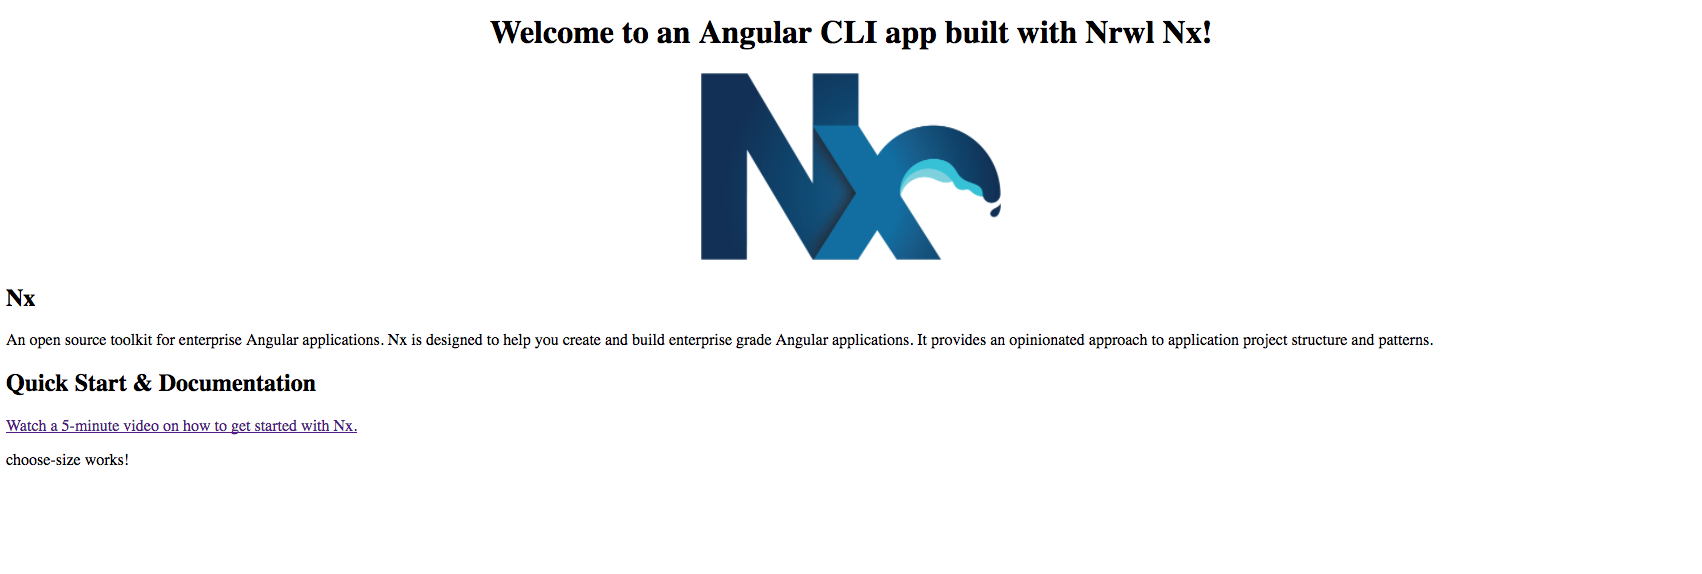
\includegraphics[width=13cm, height=9cm]{containers-and-routing/choose-size-screenshot}

\subsection{ ngrx/router-store }

Before we move any further with regards to angular routes, let's discuss
ngrx/router. In short, ngrx/router exists so that the route can be in the store
as well. By default ngrx/router will dispatch a ROUTER\_NAVIGATION action
\footnote{We'll discuss this a bit more when we get to the chapter on ngrx/store},
when a navigation route get's called. This will enable time traveling with
regards to routes.

\subsection{ Why use ngrx/router-store }

Ngrx/router-store can be advantageous in two regards. One, it adheres to the
principle of there being a single state of truth \footnote{https://redux.js.org/docs/introduction/ThreePrinciples.html\#single-source-of-truth}.
Two, it helps applications with regards to breadcrumbs, and adding filters to the
url. If one wanted to follow an architecture, where the route contains the current
state of the application(filters, inputs etc.) router-store definitely make's it
very easy to do so.

\subsection{ Adding ngrx/router-store to our app }

In order to add ngrx/router-store to our app, run:
\begin{verbatim}
  npm install @ngrx/router-store --save
\end{verbatim}

In addition, we will be adding the route to our store for the first time, so we
will be needing ngrx/store. Please run \footnote{This will also install ngrx/store-devtools + ngrx/effects}:
\begin{verbatim}
  npm install @ngrx/store --save
\end{verbatim}

In our app.module.ts we will be adding the following:
\begin{verbatim}
  + import { StoreModule } from '@ngrx/store';
  + import { StoreRouterConnectingModule, routerReducer } from '@ngrx/router-store';
  + import { StoreDevtoolsModule } from '@ngrx/store-devtools';
  // inside of imports
  + StoreModule.forRoot({
  +    router: routerReducer
  + }),
  + StoreRouterConnectingModule.forRoot({
  +   stateKey: 'router'
  + });
  + StoreDevtoolsModule.instrument({
  +    maxAge: 5
  + }),
\end{verbatim}

\subsubsection{ Side note when using devtools with ngrx/router-store }

One final note when using ngrx/store router-store with devtools. The
RouteStateSnapshot is a very large object, containing large amounts of data. I've
run across performance issues, it is therefore reccomend setting up a
custom router state serializer
\footnote{https://github.com/ngrx/platform/blob/master/docs/router-store/api.md\#custom-router-state-serializer}.
The idea is that the user provides the specific items one wants from the route.
This allows for maybe 3 key/values to appear, instead of a 1000+. For the sake of
brevity, we will not include the technical steps here. However, the code for doing
so can be found in the github branch equivalent.
